\documentclass[11pt,a4paper]{article}

\usepackage[utf8]{inputenc}
\usepackage[T1]{fontenc}
\usepackage[english]{babel}
\usepackage{geometry}
\usepackage{microtype}
\usepackage{booktabs}
\usepackage{enumitem}
\usepackage{graphicx}
\usepackage{tikz}
\usetikzlibrary{positioning, shapes.geometric, arrows.meta, backgrounds, fit}
\usepackage{hyperref}

\geometry{margin=2.6cm}
\setlist{noitemsep,topsep=2pt}

\hypersetup{
    colorlinks=true,
    linkcolor=blue,
    filecolor=magenta,      
    urlcolor=cyan,
    pdftitle={Research Project Proposal - Davide Ditolve},
    pdfpagemode=FullScreen,
}

\begin{document}

% ------------------------------------------------------------------------------
% 1) FRONTISPIECE
% ------------------------------------------------------------------------------
\section{Frontispiece}

\begin{center}
    
\includegraphics[width=0.22\textwidth]{logo_ecampus.png}\\[0.4cm]
    {\large \textsc{eCampus Telematic University}}\\[0.1cm]
    {\small PhD Program in Applied Sciences to Well-being and Sustainability (XLII Cycle)}\\[0.6cm]
    
    {\large \textbf{RESEARCH PROJECT PROPOSAL}}\\[0.3cm]
    {\Large \textbf{Optimization of Local Language Models and RAG Architectures for Decision Support in Psychopathology: An Engineering Approach to Service Sustainability and Patient Well-being}}\\[0.8cm]
\end{center}

\noindent
\textbf{Candidate:} Davide Ditolve \hfill \textbf{Research Line:} Line 4\\
\textbf{Proposed Supervisor:} Prof. Riccardo Pecori (IINF-05/A)\\[0.4cm]
\textbf{Research Line Referent Professors:}\\
{\small Bocchio Chiavetto L. (BIOS-10/A); Cavallo M. (PSIC-04/B); De Giorgio A. (PSIC-01/A); Di Fronso S. (MEDF-01/A); Di Lernia D (PSIC-01/A); Ieraci A. (BIOS-10/A); Iuliano E. (MEDF-01/A); Lombardi E. (PSIC-02/A); Marchetti B. (IIND-05/A); Miraglia F. (BIOS-06/A); Nimbi FM. (PSIC-08/B); Pedroli E. (PSIC-01/C); Picerno P. (IBIO-01/A); Tradigo G. (IINF-05/A); Vecchio F. (BIOS-06/A); Verdini F (IBIO-01/A).}

\subsection*{Abstract}
Integrating Artificial Intelligence (AI) in mental health offers opportunities to enhance diagnostic accuracy and care sustainability, provided that clinical safety and data privacy are guaranteed. This project proposes an interdisciplinary engineering approach to design and optimize a clinician-facing decision support tool based on local Large Language Models (LLMs). The system is grounded in a Retrieval-Augmented Generation (RAG) pipeline linked to official taxonomic databases (ICD-11 and DSM-5-TR) to mitigate hallucinations and clinical sycophancy. We propose a hybrid cloud-edge computational model: cloud resources support offline model training, embedding index generation, and fallback execution, while inference is run on local edge nodes to ensure data confidentiality. The study will evaluate: (1) system effectiveness in reducing diagnostic errors and clinician cognitive workload; (2) patient well-being impact through a structured ``digital anamnesis'' protocol to map dysfunctional usage of commercial chatbots.

\vspace{0.4cm}
\noindent \textbf{Keywords:} Decision Support; Local RAG; Optimized Language Models; Psychophysical Well-being; Sustainability of Care; Digital Anamnesis.

\newpage

% ------------------------------------------------------------------------------
% 2) THEORETICAL INTRODUCTION
% ------------------------------------------------------------------------------
\section{Theoretical Introduction}

Promoting the well-being of individuals with psychiatric conditions requires personalized, secure, and sustainable care models. In this context, e-health and clinical decision support systems (CDSS) offer promising solutions. However, integrating these technologies into psychopathology presents unique clinical, ethical, and technical challenges that prevent their uncritical transposition from general medicine (Cremaschi \& Pierotti, 2026).

Unlike general medicine, which is supported by biological markers, psychopathology is grounded in a clinical object that is subjective, narrative, and relational (Jaspers, 1963; Stanghellini \& Fuchs, 2013). Suffering is expressed through narrative and clinical setting dynamics (Parnas et al., 2013). Deploying Large Language Models (LLMs) to support clinical reasoning introduces critical engineering and well-being challenges:

\begin{enumerate}[label=\alph*)]
    \item \textbf{Taxonomic grounding and cognitive bias mitigation:} Generative AI systems are prone to hallucinations and sycophancy toward user hypotheses (Sharma et al., 2023), risking clinician diagnostic errors. As analyzed by Vidotto, Ditolve, and Panzeri (2026), LLMs simulate understanding without real semantic intent (the ``epistemology of simulation''). To safeguard patient well-being, the technology must act as a controlled nosographical organizer. In computer engineering, this requires developing Retrieval-Augmented Generation (RAG) systems that dynamically constrain LLM outputs to official taxonomies such as ICD-11 and DSM-5-TR (Cremaschi et al., 2025).
    
    \item \textbf{Computational safety and hybrid cloud-edge architectures:} Processing highly sensitive clinical data requires strict privacy standards (GDPR, EU AI Act). Submitting patient records to commercial cloud APIs raises severe data leakage risks and latency issues. Therefore, designing local, resource-constrained AI architectures is a priority (pervasive AI; Pecori, 2023). However, pure local execution faces memory and computational limits. We address this by introducing a hybrid edge-cloud architecture: high-capacity cloud services are used offline for model training, fine-tuning, and embedding indexing, while clinical inference is run locally on edge nodes to ensure data isolation.
    
    \item \textbf{The relational dimension and AI as the ``third in the room'':} Patients increasingly use commercial chatbots as therapeutic surrogates (Cremaschi \& Pierotti, 2026). This unregulated interaction can trigger cybercondria, dependency, or isolation (Dohnány et al., 2026). It is therefore crucial to integrate this digital experience into the therapeutic relationship through a structured ``digital anamnesis'' protocol, mapping patient chatbot interaction patterns as informative data features.
\end{enumerate}

% ------------------------------------------------------------------------------
% 3) RESEARCH OBJECTIVES AND HYPOTHESES
% ------------------------------------------------------------------------------
\section{Research Objectives and Hypotheses}

\subsection{Synergy between Technology and Well-being}
In this project, computer engineering solutions are specifically designed to safeguard clinical safety and patient well-being:
\begin{itemize}
    \item \textbf{Clinical reliability via nosographical constraints:} Minimize diagnostic errors stemming from LLM hallucinations by enforcing adherence to official diagnostic criteria through a RAG pipeline.
    \item \textbf{Architectural security and data protection:} Safeguard sensitive patient information via local inference execution, minimizing data transmission risks.
    \item \textbf{Clinical integration of digital experiences (Digital Anamnesis):} Incorporate patients' digital interactions with AI into the therapeutic setting, utilizing these patterns as clinical insights.
\end{itemize}

\subsection{Specific Objectives}
\begin{enumerate}
    \item \textbf{Design and optimization of the decision support system (CDSS):} Develop a clinician-facing software architecture integrating local LLMs and ICD-11/DSM-5-TR taxonomies, utilizing a hybrid edge-cloud setup to optimize compute workloads and performance.
    \item \textbf{Clinical-relational study of patient-AI interaction:} Validate a structured ``digital anamnesis'' protocol to assess chatbot influence on the therapeutic alliance and patient well-being, mapping dysfunctional usage profiles.
    \item \textbf{Experimental evaluation of system performance:} Quantitatively evaluate the system's efficacy in reducing diagnostic errors alongside its computational efficiency (latency, memory footprint, and RAG retrieval/generation quality).
    \item \textbf{Governance and Data Privacy guidelines:} Draft operational recommendations for safe AI adoption in mental health services, compliant with the EU AI Act and GDPR.
\end{enumerate}

\subsection{Research Hypotheses}
\begin{itemize}
    \item \textbf{H1 (Decision Support and Grounding):} Clinicians using the optimized local RAG CDSS (Independent Variable) will show significantly higher diagnostic accuracy and a lower rate of nosographical omission errors (Dependent Variables) compared to manual consultation, while maintaining an equivalent or lower cognitive workload (NASA-TLX).
    \item \textbf{H2 (Interaction and Well-being):} Patients exhibiting a dysfunctional or compulsive chatbot usage profile (Independent Variable, measured via Digital Anamnesis) will show lower therapeutic alliance scores (WAI scale compiled by both patient and clinician) and higher baseline symptom severity (BDI-II, BAI) (Dependent Variables) than patients with controlled or no chatbot usage.
    \item \textbf{H3 (Efficiency and Sustainability):} The optimized hybrid edge-cloud architecture (local quantized LLM inference with cloud training and fallback) will achieve latency (time-to-first-token < 500ms) and throughput (> 15 tokens/sec) suitable for clinical utility, reducing clinician cognitive load compared to cloud-only execution, without compromising RAG faithfulness (Ragas evaluation).
\end{itemize}

% ------------------------------------------------------------------------------
% 4) METHODOLOGY
% ------------------------------------------------------------------------------
\section{Methodology}

The project adopts an interdisciplinary mixed-methods research design, split between a computer engineering component for system development and optimization, and a clinical-experimental component to evaluate patient well-being impact.

\subsection{Study Type and Experimental Design}
\begin{itemize}
    \item \textbf{CDSS Evaluation (Phase 1):} Controlled study with a within-subjects (cross-over) design. Clinicians will evaluate complex cases under two conditions: (a) supported by the optimized CDSS; (b) via manual text consultation.
    \item \textbf{Observational Study on the Relationship (Phase 2):} Correlational study on patients to analyze the relationship between AI usage profiles (via Digital Anamnesis), therapeutic alliance (WAI scale), and well-being.
    \item \textbf{Action Research on Care Quality (Phase 3):} Focus groups with healthcare workers to identify barriers to adoption and define organizational sustainability metrics.
\end{itemize}

\begin{figure}[htbp]
    \centering
    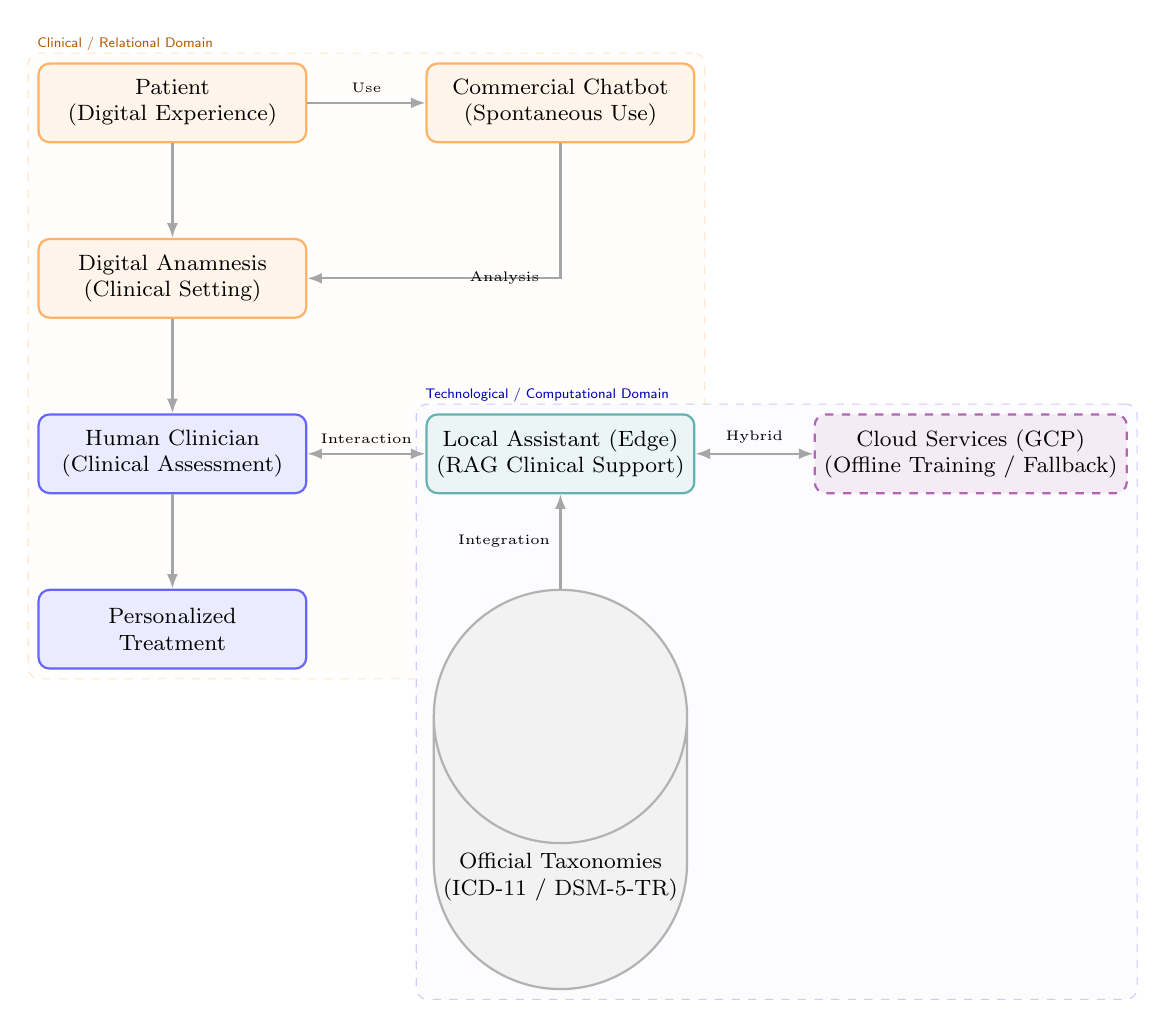
\begin{tikzpicture}[
        node distance=1.2cm and 1.5cm,
        patient_node/.style={draw, rectangle, rounded corners=4pt, minimum width=3.4cm, minimum height=1.0cm, align=center, fill=orange!8, draw=orange!60, thick, font=\footnotesize},
        clinician_node/.style={draw, rectangle, rounded corners=4pt, minimum width=3.4cm, minimum height=1.0cm, align=center, fill=blue!8, draw=blue!60, thick, font=\footnotesize},
        tech_edge_node/.style={draw, rectangle, rounded corners=4pt, minimum width=3.4cm, minimum height=1.0cm, align=center, fill=teal!8, draw=teal!60, thick, font=\footnotesize},
        tech_cloud_node/.style={draw, rectangle, rounded corners=4pt, minimum width=3.4cm, minimum height=1.0cm, align=center, fill=violet!8, draw=violet!60, thick, dashed, font=\footnotesize},
        database_node/.style={draw, cylinder, shape border rotate=90, minimum width=2.4cm, minimum height=1.0cm, align=center, fill=gray!10, draw=gray!60, thick, font=\footnotesize},
        arrow/.style={-{Latex[scale=0.8]}, thick, draw=gray!70},
        bi_arrow/.style={<->, {Latex[scale=0.8]}-{Latex[scale=0.8]}, thick, draw=gray!70}
    ]
        % Nodes
        \node (patient) [patient_node] {Patient\\(Digital Experience)};
        \node (chatbot) [patient_node, right=of patient] {Commercial Chatbot\\(Spontaneous Use)};
        \node (anamnesis) [patient_node, below=of patient] {Digital Anamnesis\\(Clinical Setting)};
        \node (clinician) [clinician_node, below=of anamnesis] {Human Clinician\\(Clinical Assessment)};
        \node (support) [tech_edge_node, right=of clinician] {Local Assistant (Edge)\\(RAG Clinical Support)};
        \node (cloud) [tech_cloud_node, right=of support] {Cloud Services (GCP)\\(Offline Training / Fallback)};
        \node (kb) [database_node, below=of support] {Official Taxonomies\\(ICD-11 / DSM-5-TR)};
        \node (treatment) [clinician_node, below=of clinician] {Personalized\\Treatment};

        % Arrows
        \draw [arrow] (patient) -- node[anchor=south, font=\tiny] {Use} (chatbot);
        \draw [arrow] (chatbot) |- node[anchor=west, pos=0.7, font=\tiny] {Analysis} (anamnesis);
        \draw [arrow] (patient) -- (anamnesis);
        \draw [arrow] (anamnesis) -- (clinician);
        \draw [arrow] (clinician) -- (treatment);
        \draw [bi_arrow] (clinician) -- node[anchor=south, font=\tiny] {Interaction} (support);
        \draw [arrow] (kb) -- node[anchor=east, font=\tiny] {Integration} (support);
        \draw [bi_arrow] (support) -- node[anchor=south, font=\tiny] {Hybrid} (cloud);

        % Groups
        \begin{scope}[on background layer]
            \node (clinical_group) [fill=orange!1, draw=orange!20, dashed, rounded corners, fit=(patient) (chatbot) (anamnesis) (clinician) (treatment)] {};
            \node (tech_group) [fill=blue!1, draw=blue!20, dashed, rounded corners, fit=(support) (cloud) (kb)] {};
            \node at (clinical_group.north west) [anchor=south west, font=\tiny\sffamily, text=orange!70!black, yshift=-0.1cm] {Clinical / Relational Domain};
            \node at (tech_group.north west) [anchor=south west, font=\tiny\sffamily, text=blue!70!black, yshift=-0.1cm] {Technological / Computational Domain};
        \end{scope}
    \end{tikzpicture}
    \caption{Clinical-Technological Workflow and Intervention Design}
    \label{fig:workflow}
\end{figure}

\subsection{Technological Architecture and Model Optimization (IINF-05/A)}
The CDSS is designed as a layered software architecture optimized for deployment under local computing resource constraints and strict health data privacy limits:
\begin{itemize}
    \item \textbf{Local Inference and Quantization:} To guarantee patient privacy, clinical inference is executed locally using optimized runtimes (e.g., llama.cpp/Ollama). To run large language models (e.g., Llama-3-8B) on consumer-grade clinical workstations (pervasive AI; Pecori, 2023), post-training quantization (PTQ) techniques in GGUF format (4-bit and 8-bit, e.g., Q4\_K\_M and Q8\_0) will be applied, reducing VRAM usage while preserving reasoning capabilities.
    \item \textbf{Hybrid Computing and Cloud Support:} To overcome edge computing limitations, we introduce a hybrid service model. Cloud services (e.g., Google Cloud Platform) will be utilized for high-compute asynchronous tasks that do not expose patient data: (1) offline training and parametric fine-tuning (e.g., LoRA); (2) vector indexing of the ICD-11 taxonomy; (3) large-scale synthetic benchmarking. Additionally, the cloud will serve as encrypted fallback computation in case of edge hardware overload.
    \item \textbf{RAG Pipeline and Grounding:} Grounding the LLM to ICD-11/DSM-5-TR is achieved via hierarchical RAG. Nosological categories are indexed in a local vector database (pgvector) preserving parent-child relations. Retrieval employs hybrid search (dense semantic embeddings via BioLinkBERT combined with sparse BM25 lexical search). A prompt routing module will orchestrate queries to selectively retrieve diagnostic criteria and exclusions.
    \item \textbf{Technical Performance Metrics:} System performance will be evaluated using: (1) efficiency metrics: latency (\textit{time-to-first-token} in ms), throughput (\textit{tokens/second}), and memory footprint; (2) RAG quality metrics: faithfulness, answer relevance, and context recall, calculated via frameworks such as Ragas.
\end{itemize}

\subsection{Study Variables}
\begin{itemize}
    \item \textbf{Independent Variables:}
    \begin{itemize}
        \item \textit{Support Condition:} Use of the clinician-facing CDSS vs. Traditional consultation of manuals.
        \item \textit{Patient's AI Use Profile:} Dysfunctional/compulsive use vs. Informative/moderate use vs. Non-use.
    \end{itemize}
    \item \textbf{Dependent Variables:}
    \begin{itemize}
        \item \textit{Diagnostic accuracy:} percentage of match with the gold standard diagnosis.
        \item \textit{Diagnostic error rate:} frequency of omitted criteria or missed differential diagnoses.
        \item \textit{Clinician's mental workload:} score on the NASA-TLX scale.
        \item \textit{Quality of the therapeutic alliance:} score on the Working Alliance Inventory (WAI) scale.
        \item \textit{Patient's psychophysical well-being:} score on the Outcome Questionnaire-45 (OQ-45) scale.
    \end{itemize}
\end{itemize}

\subsection{Sample Selection and Inclusion/Exclusion Criteria (Feasibility)}
\begin{itemize}
    \item \textbf{Clinician Sample:} Recruitment will occur via convenience sampling. A group of mental health professionals (clinical psychologists, psychotherapists, and psychiatrists) of \textbf{scientifically significant size} will be involved to ensure adequate statistical power for within-subjects analyses.
    \begin{itemize}
        \item \textit{Inclusion:} Registration in the Register; active practice (at least 10 hours per week); signed informed consent.
        \item \textit{Exclusion:} Lack of minimal familiarity with digital interfaces; direct involvement in the tool's development phase.
    \end{itemize}
    
    \item \textbf{Patient Sample:} Enrollment will occur at partner clinical services, subject to Ethical Committee approval. A sample of patients of \textbf{scientifically significant size} will be selected to ensure adequate statistical power.
    \begin{itemize}
        \item \textit{Inclusion:} Age 18-65 years; currently under the care of the clinical service; declared spontaneous use of chatbots for health in the last 6 months; signed informed consent.
        \item \textit{Exclusion:} Severe cognitive deficits or neurological disorders; acute-phase psychotic spectrum disorders; active suicidal ideation or imminent self-harm risk.
    \end{itemize}
    
    \item \textbf{Materials (Clinical Vignettes):} A set of standardized and validated clinical vignettes (e.g., \textit{DSM-5-TR Casebook}) will be employed in a \textit{scientifically significant quantity} to allow a balanced and statistically relevant coverage of the different nosographical macro-areas.
\end{itemize}

\subsection{Data Collection Tools}
\begin{itemize}
    \item \textbf{Clinical Evaluation (Phase 1):} Diagnostic accuracy scores; \textit{NASA-TLX} scale for mental workload; \textit{SUS} for the tool's usability.
    \item \textbf{Relational Evaluation (Phase 2):} Structured \textit{Digital Anamnesis} interview (Cremaschi \& Pierotti, 2026); \textit{WAI} scale completed by the patient (WAI-C) and therapist (WAI-T); standardized clinical scales (\textit{BDI-II} for depression, \textit{BAI} for anxiety, \textit{OQ-45} for general well-being).
    \item \textbf{Quality of Care (Phase 3):} Treatment clinical appropriateness evaluation grid (completed by independent judges in a blind manner); tracking sheet for diagnostic omission errors.
\end{itemize}

\subsection{Data Analysis}
\begin{itemize}
    \item \textbf{Quantitative Analysis:} Paired t-test (or non-parametric Wilcoxon equivalent) to compare accuracy, error, and mental workload (Phase 1). Correlation analysis and linear regression models to verify the impact of the AI use profile (Phase 2) on the therapeutic alliance and the patient's general well-being.
    \item \textbf{Qualitative Analysis:} Thematic analysis of focus group transcriptions with clinicians to map organizational factors and clinical areas of greatest utility for the tool.
\end{itemize}

% ------------------------------------------------------------------------------
% 5) EXPECTED RESULTS
% ------------------------------------------------------------------------------
\section{Expected Results}

The research aims to produce concrete results for clinical practice and service management:
\begin{enumerate}
    \item \textbf{Evidence on decision support efficacy:} Empirical demonstration of how a clinician-facing tool can support diagnostic precision, reduce systemic errors, and improve the quality of care.
    \item \textbf{Validation of Digital Anamnesis:} Release of a validated digital anamnesis sheet, usable by clinicians to understand the impact of commercial chatbot use on patient well-being.
    \item \textbf{Care Governance and Sustainability Model:} Definition of guidelines and risk matrices for the safe adoption of AI in healthcare services, promoting more effective, consistent, and economically sustainable therapeutic pathways.
    \item \textbf{Selectivity and clinical error reduction:} Quantitative estimation of the decrease in diagnostic errors (omissions, missed differentials) due to the tool's use.
    \item \textbf{Scientific dissemination:} Publication of at least 3 articles in indexed scientific journals (e.g., \textit{JMIR}, \textit{Frontiers}) and presentations at national and international congresses.
\end{enumerate}

% ------------------------------------------------------------------------------
% 6) PROJECT INNOVATIVENESS
% ------------------------------------------------------------------------------
\section{Project Innovativeness}

The project's innovativeness lies in overcoming the strictly technological approach of clinical AI by proposing an interdisciplinary paradigm shift where computer engineering acts as the secure backbone enabling clinical well-being.

\subsection{Engineering Innovation and Edge-Cloud Hybrid Architecture}
Most e-health applications rely on cloud APIs, raising serious concerns regarding health data privacy (GDPR, EU AI Act). This project stands out by implementing a resource-constrained hybrid architecture (pervasive AI; Pecori, 2023). Optimizing local execution on clinical workstations while offloading non-sensitive training and indexing tasks to the cloud represents a technical innovation that guarantees both legal and economic sustainability for digital health services.

\subsection{Epistemological Innovation and Nosographical Grounding}
Unlike standard ML approaches treating LLMs as predictive black boxes, the project introduces a theoretical-technical innovation grounded in the ``epistemology of simulation'' (Vidotto, Ditolve \& Panzeri, 2026). Since LLMs simulate cognitive activity without real semantic comprehension, the system is designed to serve as a ``cognitive mirror'' and nosographical organizer rather than a clinician replacement. This ensures that clinical responsibility remains entirely with the human clinician.

\subsection{Relational Innovation: Digital Anamnesis in the Clinical Setting}
The project is innovative in defining and validating a formal \textit{Digital Anamnesis} protocol to address patients' spontaneous use of commercial chatbots. By viewing conversational AI as a ``new relational and transitional object'' (Cremaschi \& Pierotti, 2026), this research provides therapists with structured tools to map and address dysfunctional interaction patterns (cybercondria, isolation), preventing therapeutic alliance deterioration.

\subsection{Interdisciplinary Synergy for Care Sustainability}
The project represents a concrete convergence between clinical psychology/psychometrics (research lines 4 and 5) and computer engineering (SSD IINF-05/A). Care sustainability is redefined as care quality sustainability: computer engineering provides the secure, optimized infrastructure that reduces diagnostic error and cognitive load, enabling personalized clinical pathways that safeguard patient well-being.

% ------------------------------------------------------------------------------
% 7) ESSENTIAL BIBLIOGRAPHY
% ------------------------------------------------------------------------------
\section{Essential Bibliography}

\begin{enumerate}[label={[\arabic*]}]
    \item Abràmoff, M. D., Lavin, P. T., \& Folk, J. C. (2018). Pivotal trial of an autonomous AI-based diagnostic system for detection of diabetic retinopathy in primary care offices. \textit{npj Digital Medicine}, 1(1), 39.
    \item Bordin, E. S. (1979). The generalizability of the psychoanalytic concept of the working alliance. \textit{Psychotherapy: Theory, Research \& Practice}, 16(3), 252.
    \item Cremaschi, M., \& Pierotti, A. P. (2026). Intelligenza artificiale in psicopatologia: epistemologia clinica, relazione terapeutica e governance. \textit{Frontiers in Digital Health} (under review).
    \item Cremaschi, M., Ditolve, D., et al. (2025). Decoding clinical reasoning: a local Retrieval-Augmented Generation approach on ICD-11 for mental health support. \textit{LLMind1 Pilot Study} (preprint).
    \item Dohnány, S., Kurth-Nelson, Z., et al. (2026). Technological folie à deux: Feedback loops between AI chatbots and mental illness. \textit{Nature Mental Health}, doi:10.48550/arXiv.2507.19218.
    \item Finn, S. E. (2007). \textit{In Our Clients' Shoes: Theory and Techniques of Therapeutic Assessment}. Lawrence Erlbaum Associates.
    \item Flückiger, C., Del Re, A. C., \& Horvath, A. O. (2018). The alliance in adult psychotherapy: A meta-analytic synthesis. \textit{Psychotherapy}, 55(4), 316-340.
    \item Jaspers, K. (1963). \textit{General Psychopathology}. University of Chicago Press.
    \item Kendler, K. S. (2016). The nature of psychiatric disorders. \textit{World Psychiatry}, 15(1), 5-12.
    \item Parnas, J., Sass, L. A., \& Zahavi, D. (2013). Rediscovering psychopathology: The epistemology and phenomenology of the psychiatric object. \textit{Schizophrenia Bulletin}, 39(2), 270-277.
    \item Pecori, R. (2018). A Virtual Learning Architecture Enhanced by Fog Computing and Big Data Streams. \textit{Future Internet}, 10(12), 120.
    \item Pecori, R. (2023). Pervasive and Resource-Constrained Artificial Intelligence in Healthcare: Applications in E-Health and Clinical Decision Support. \textit{Proceedings of the PeRConAI Workshop}.
    \item Ribeiro, A. H., et al. (2020). Automatic diagnosis of the 12-lead ECG using a deep neural network. \textit{Nature Communications}, 11(1), 1760.
    \item Sander, L. W. (2008). \textit{Living Systems, Evolving Consciousness, and the Emerging Person}. Analytic Press.
    \item Sharma, M., et al. (2023). Towards understanding sycophancy in language models. \textit{arXiv preprint arXiv:2310.13548}.
    \item Stanghellini, G., \& Fuchs, T. (eds.) (2013). \textit{One Century of Karl Jaspers' General Psychopathology}. Oxford University Press.
    \item \textbf{Vidotto, G., Ditolve, D., \& Panzeri, A. (2026). Una riflessione critica sui Large Language Models in psicologia clinica: Malfunzionamento, metacognizione, memoria ed etica. \textit{PCC}, 2026(2).}
    \item World Health Organization. (2024). \textit{Ethics and Governance of Artificial Intelligence for Health: Guidance on Large Multi-Modal Models}. WHO Guidelines.
\end{enumerate}

\end{document}

The above content shows the entire, complete file contents of the requested file.